

\section{Software} \label{sec:software}

Para reemplazar el rol que cumplía el \textit{software} FelixGX en el espectrofluorímetro original desarrollamos, junto con Hernán Grecco, dos paquetes de Python de control de instrumental y adquisición de datos \cite{napoli_tdinapoli_2024,grecco_hgrecco_2024}.
El código corre en la CPU de la RP y permite controlar al espectrofluorímetro a través de una interfaz de programación de aplicaciones (API) y una interfaz gráfica simple (GUI) desarrollada con el paquete \textit{Jupyter Widgets} de \textit{IPython}.
El programa conformado por ambos paquetes está compuesto de cuatro capas principales (\textbf{Fig. \ref{fig:code}}):

\begin{itemize}
     \item \textbf{RedpiPy}: Es uno de los dos paquetes que desarrollamos. Consiste en un \textit{wrapper} (llamado \textit{rpwrap}) de la API original de la RP que resulta en que el código esté mejor organizado para hacer una aplicación en Python. Se compone de funciones y clases que permiten manejar el \textit{hardware} de la RP a bajo nivel, como \textit{RPDO} que controla los pines digitales, así como algunas clases de más alto nivel como \textit{Oscilloscope} que permite manejar el osciloscopio.
     \item \textbf{Clases de dispositivos}: Controlan componentes individuales del espectrofluorímetro, como los monocromadores, el láser pulsado, y los motores de los monocromadores permitiendo el control de todas las partes por separado. 
     \item \textbf{Clase Spectrometer}: Coordina el \textit{hardware} para protocolos de medición específicos (por ejemplo, adquirir un espectro de emisión). Es fácil de usar desde un script en Python o desde la línea de comandos. Además, es la encargada de contar los pulsos de voltaje negativo registrados por el PMT (ver sección \ref{sec:conteo}). Es utilizada por la interfaz gráfica.
     \item \textbf{Interfaz gráfica (GUI)}: proporciona herramientas de adquisición similares a las de FelixGX. Se accede a través de la web y utiliza el paquete \textit{Jupyter Widgets} de \textit{IPython}.
\end{itemize}

Gracias a este diseño la parte del código que implementa el control del instrumento es completamente general y está desacoplada del resto, por lo que debería funcionar para cualquier modelo de espectrofluorímetro cuyos monocromadores sean controlados por motores por paso, y la señal de luminiscencia se lea con un PMT.
Por otro lado, la API pública le permite al usuario avanzado crear sus propios protocolos de medición que se pueden ejecutar sin la supervición de un operario.
Tanto \textit{RedpiPy} como \textit{RefurbishedPTI} (el paquete que controla al espectrofluorímetro) se encuentran públicos en repositorios de \href{https://github.com}{GitHub} con sus respectivas instrucciones de instalación. 
El apéndice \ref{apendice:instrucciones_uso} explica detalladamente algunos ejemplos que muestran cómo medir un espectro estacionario y el tiempo de vida para distintas longitudes de onda, ambos a través de la API y de la GUI.
En las próximas secciones explicaremos cuál es el protocolo del software para hacer mediciones espectrales estáticas y dinámicas, independientemente de la interfaz que se use para obtenerlas.


%\todo{ \\
%capacidades del software \\
%\\
%Jerarquía de clases API para desacoplar. Extensión del software: sirve para espectrofluorímetro genérico siempre y cuando tengas motor por pasos y pmt.\\
%\\
%quien cuenta los picos, (mencionar que hay analisis de picos más adelante)\\
%\\
%Modos de uso, API GUI (capacidades, más detallado en apéndice).\\
%}

\begin{figure}[t]
     \centering
     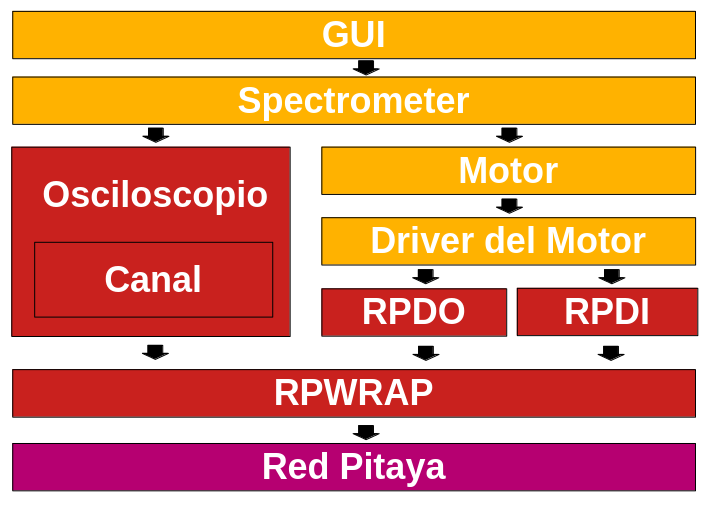
\includegraphics[width=0.8\textwidth]{software-diagram.png}
     \caption{\textbf{Estructura del \textit{software}}. Cada elemento del \textit{software} está ordenado de alto nivel (arriba) a bajo nivel (abajo). En amarillo se ven las componentes de \textit{refurbishedPTI}, en rojo las de \textit{redpipy}, en rosa la API y el \textit{hardware} de la RP.}
     \label{fig:code}
\end{figure}

%\todo{introduccion a medicion de tiempos de vida}

%El tiempo máximo de adquisición de 8 ms ofrece una ventana suficientemente amplia para la mayoría de los materiales luminiscentes. 
%Como se mencionó anteriormente, cuando se requiere medir tiempos de vida mucho más largos al tiempo de adquisición máximo (0.5 ms), la ventana de detección puede desplazarse respecto al \textit{trigger} para cubrir un rango más amplio. 
%El \textit{software} permite configurar la cantidad de veces que se mide cada ventana de 0.5 ms, lo que hace posible construir una curva de decaimiento más extensa de la luminiscencia.

%\todo{ \\
%explicar que es lo mismo que antes salvo que se usa el trigger.\\
%Explicar funcionamiento de las pantallas y offsets \\
%}

\section{Protocolo de medición estática}

El espectro estático de emisión(excitación) de una muestra consiste en la medición de su intensidad de luminiscencia al iluminar(observar) en una longitud de onda fija, y observar(iluminar) barriendo un rango de longitudes de onda.
Por lo tanto, antes de iniciar una medición deben estar definidos sus parámetros que en este caso son el tiempo de integración $t_{int}$, la longitud de onda de iluminación(medición) $\lambda_e$, y la longitud de onda inicial $\lambda_i$ y final $\lambda_f$ del barrido, así como el paso $\lambda_s$ entre cada medición de intensidad.
En el caso de tomar un espectro de UCNPs, dado que la iluminación proviene del diodo láser de 976 nm, también es necesario configurar la potencia óptica de excitación.

Una vez configurados los parámetros, el espectrofluorímetro debe realizar los siguientes pasos:

\begin{enumerate}
     \item \textbf{Inicializar los monocromadores} haciendo girar los motores en una misma dirección hasta que la señal del fin de carrera de cada uno sea de 5 V. Esto sirve para que la longitud de onda guardada por el \textit{software} coincida con la real.
     \item \textbf{Mover el monocromador estático} de emisión(excitación) hasta $\lambda_e$. 
     \item \textbf{Mover el monocromador dinámico} de excitación(emisión) hasta $\lambda_f$ en pasos de $\lambda_s$. Para cada longitud de onda los pasos (a) y (b) se deben repetir  $n$ veces, donde $n$ es tal que $n \times t_{max} \geq t_{int}$ y $t_{max}$ es el máximo tiempo de medición que soporta la RP (0.5 ms):
     \begin{enumerate}
          \item Medir la señal del PMT (\textbf{Fig. \ref{fig:diag_medicion_estatica}A}).
          \item Contar los picos en esa señal (ver sección \ref{sec:conteo}) y acumularlos. Al finalizar, el resultado es la cantidad de picos (fotones) contados por segundo.
     \end{enumerate}
\end{enumerate}

\noindent Una vez que el monocromador dinámico llega a $\lambda_f$ la cantidad de cuentas por segundo para cada longitud de onda se guarda en una tabla y termina la medición.
Al caracterizar UCNPs la excitación se da a través del láser externo, por lo que se deben configurar sus parámetros independientemente y el monocromador de excitación, que selecciona la longitud de onda de la lámpara que ilumina a la muestra, no toma ningún rol.
Como siempre se miden pantallas enteras, los tiempos de integración posibles son múltiplos de 0.5 ms.
Esto no es un problema porque los tiempos de integración necesarios suelen ser típicamente del orden de los segundos, dos o tres órdenes de magnitud mayores a la duración de la pantalla.
Además, la tabla de datos resultante de una medición contiene el tiempo de integración para cada punto con un error de $\sim 15$ ns.
En caso de que sea necesario medir con un tiempo de integración más preciso, esto se puede lograr modificando levemente el \textit{software} de \textit{refurbishedPTI}.

\begin{SCfigure}
     \centering
     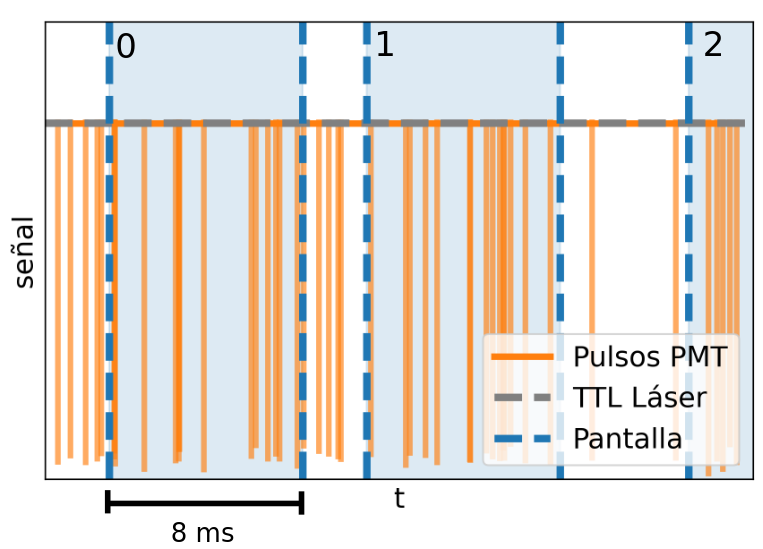
\includegraphics[width=0.6\textwidth]{diag_medicion_estatica.png}
     \caption{\textbf{Diagrama de medición estática.} En naranja se ve la señal del PMT. La línea punteada gris alta indica que el láser está en modo CW. En azul se ven las ventanas de la señal que lee la RP.}
     \label{fig:diag_medicion_estatica}
\end{SCfigure}


\section{Protocolo de medición dinámica} \label{sec:proceso_dinamico}

La medición de los tiempos de vida de las nanopartículas de \textit{upconversion} se realiza mediante la técnica de TCSPC (ver sección \ref{sec:intro_tcspc}).
Dado que estos tiempos de vida están en el rango de cientos de microsegundos, no son necesarios varios de los componentes de electrónica rápida típicos de la TCSPC utilizada en mediciones en el rango de nanosegundos, como el CFD y el TAC, los cuales son reemplazados por componentes más simples y menos costosos.
Contradictoriamente, esto hace que no se puedan caracterizar UCNPs utilizando equipos de fluorescencia de uso general, dado que el tiempo total de adquisición necesario difiere en órdenes de magnitud.
En nuestro caso, llevamos a cabo la técnica utilizando el trigger configurable a través de las entradas analógicas de la RP, y la señal TTL proveniente de la fuente de alimentación del láser.
Otra diferencia con TCSPC tradicional es el modo de excitación de la muestra.
Como la mayoría de fluoróforos orgánicos presentan su luminiscencia a través de la excitación de transiciones dipolares eléctricas, pérdia de energía por fonones, y re-emisión a través de otra transición dipolar, todos fenómenos que ocurren en el orden de los nanosegundos, es posible estudiar su espectro dinámico al excitar con un pulso del láser.
En el caso de las UCNPs, su luminiscencia se da por la dinámica no lineal de la interacción entre sus dopantes lantánidos (Yb$^{+3}$ y Er$^{+3}$), procesos que incluyen la excitación sucesiva sus electrones y por lo tanto ocurren en el orden de los microsegundos.
Por este motivo, es necesario iluminar a la muestra por algunos milisegundos para asegurarse de llegar al estado estacionario del sistema antes de medir su decaimiento.
Esto se hace aprovechando la función de alimentación pulsada (\textit{Quasi Continuous Wave} ó QCW) que ofrece la fuente ITC4020, la cual permite configurar frecuencia de pulsado $\nu$, y ciclo de trabajo $dc$ (\textbf{Fig. \ref{fig:diag_medicion_dinamica}}).

\begin{figure}
     \centering
     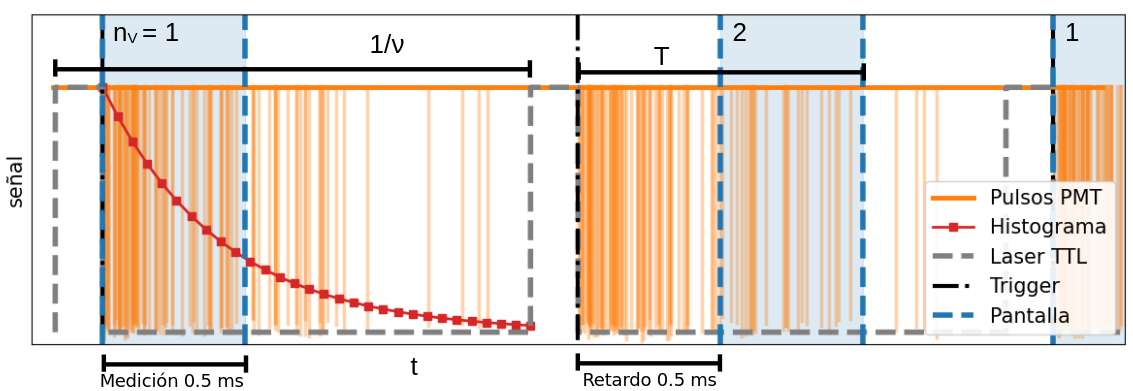
\includegraphics[width=\textwidth]{diag_medicion_dinamica.png}
     \caption{\textbf{Diagrama de medición dinámica.} La muestra es excitada intermitentemente con el láser (gris punteado). Al apagarse, el trigger de la RP se ejecuta y comienza a medir (azul) la señal (naranja) luego de esperar por $t_{ret}$. El resultado es un histograma (rojo) con la cantidad de fotones que llegaron en cada intervalo de tiempo.}
     \label{fig:diag_medicion_dinamica}
\end{figure}

Para hacer una medición de TCSPC es necesario definir la longitud de onda $\lambda$ en la que se detectará la emisión, el intervalo de tiempo $T$ en el que se van a contar los fotones luego del trigger, y la cantidad de veces $N$ que se va a medir ese intervalo.
Alternativamente, se podría definir un número de fotones $N_{fot}$ al que se quiere llegar, y medir el intervalo $T$ hasta que la cantidad de fotones medidos $n$ sea mayor a $N_{fot}$.
El protocolo por defecto de nuestro \textit{software} requiere determinar $N$.
Además, el intervalo de tiempo $T$ en el que se mide después del \textit{trigger} debe ser un múltiplo del tiempo máximo que puede medir la RP por ventana, $t_{max} = 0.5$ ms.
Por este motivo, en vez de especificar $T$, vamos a especificar $N_V$, el número de ventanas que queremos medir después del \textit{trigger} (\textbf{Fig. \ref{fig:diag_medicion_dinamica}}).
Entonces, el protocolo para realizar la medición es:

\begin{enumerate}
     \item \textbf{Inicializar los monocromadores} de forma análoga a la explicada en la sección anterior.
     \item \textbf{Mover el monocromador} de emisión hasta $\lambda$.
     \item \textbf{Iniciar el láser en modo QCW} y configurarlo para que se prenda y se apague con frecuencia $\nu$ y ciclo de trabajo $dc$.
     \item \textbf{Configurar la RP} para que espere un trigger en el canal analógico adecuado antes de medir.
     \item \textbf{Configurar un tiempo de retardo} $t_{ret} = (n_v - 1) \times t_{max}$, donde $1 \leq n_V \leq N_V$. $t_{ret}$ es el tiempo que la RP pasa sin medir después del \textit{trigger} para poder mover la ventana de medición (\textbf{Fig. \ref{fig:diag_medicion_dinamica}}). Repetir $N$ veces:
     \begin{enumerate}
          \item \textbf{Adquirir una ventana} después del \textit{trigger} y $t_{ret}$.
          \item \textbf{Encontrar los tiempos de llegada} de los pulsos usando el algoritmo explicado en la sección \ref{sec:conteo} y acumularlos.
     \end{enumerate}
     Al finalizar, el resultado es una tabla con los tiempos en los que llegaron los fotones después del \textit{trigger}.
\end{enumerate}

Con la tabla de datos final se construye un histograma (\textbf{Fig. \ref{fig:diag_medicion_dinamica}}), al cual se le puede ajustar un modelo de decaimiento para obtener el tiempo de vida de las partículas.
